\documentclass{article}
\usepackage{graphicx}
\usepackage{amsmath}
\usepackage[parfill]{parskip}
\usepackage{hyperref}
\usepackage{tikz}
\graphicspath{ {./figures/} }

\usepackage{biblatex}
\addbibresource{references.bib}

\title{COMP.SEC.220 Security Protocol\footnote{github --- \url{https://github.com/ancuongnguyen07/SecurityProtocol}}}
\author{Cuong Nguyen --- Coursework 1}
\date{22/04/2022}

\begin{document}
    
\maketitle

\section*{Exercise 1 --- XOR Encryption}
%
Given a message \emph{m} and the OTP encryption \emph{c}, we \textbf{can} compute
the OTP key \emph{k} by XORing the plaintext \emph{m} and the ciphertext \emph{c}.
The ciphertext is given by:

\begin{align*}
    c = m \oplus k,
\end{align*}

therefore, we can easily compute the \emph{k} by:

\begin{align*}
    k = c \oplus m,
\end{align*}

where \emph{c} and \emph{m} are known.

\section*{Exercise 2 --- Substitution Cipher}
%

\section*{Exercise 3 --- Diffie-Hellman}
%
\subsection*{a)}
Alice's intermediate values:

\begin{align*}
    X &= g^{a} \mod p\\
    X &= 7^6 \mod 11\\
    X &= 4 \mod 11
\end{align*}

Bob's intermediate values:

\begin{align*}
    Y &= g^{b} \mod p\\
    Y &= 7^9 \mod 11\\
    Y &= 8 \mod 11
\end{align*}

The final key that Alice and Bob exchange:

\begin{align*}
    K_{AB} &= X^b \mod p\\
    K_{AB} &= 4^9 \mod 11\\
    K_{AB} &= 3 \mod 11
\end{align*}

\subsection*{b)}
Since \(g=7\) is the primitive root of \(p=11\) so we can brute-force
\emph{a} in \(g^a = 5 \mod 11\) in at most 10 trials. Hence, the secret
value of Alice \emph{a} is 2. The secret value of Bob \emph{b}, which is 5, can be
computed by the same approach. Thus, the final key that Alice and Bob exchanged
is given by:

\begin{align*}
    K_{AB} &= X^b = Y^a = g^{ab} \mod p\\
    K_{AB} &= 1 \mod 11 
\end{align*}

\subsection*{c)}
By running the Caesar decryption script with the shift key is 1 (left-shift 1
in this case. In other words, it is right-shift 25), I obtained the plaintext:

\begin{center}
    \textbf{SUEDE JACKET WITH CANDY STRIPE LINING}
\end{center}


\section*{Exercise 4 --- Three party Diffie-Hellman}
%
Waiting for the TA's feedback

\section*{Exercise 5 --- Symmetric Encryption}
%
\begin{figure}
    \centering

    \tikzset{every picture/.style={line width=0.75pt}} %set default line width to 0.75pt        

    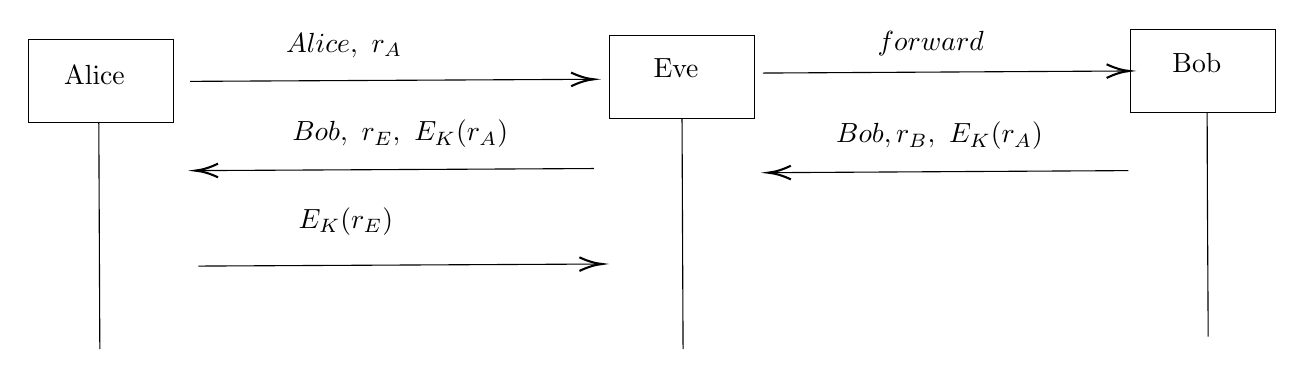
\begin{tikzpicture}[x=0.75pt,y=0.75pt,yscale=-1,xscale=1]
    %uncomment if require: \path (0,230); %set diagram left start at 0, and has height of 230

    %Shape: Rectangle [id:dp1743019806713867] 
    \draw   (32,32) -- (102,32) -- (102,72) -- (32,72) -- cycle ;

    %Shape: Rectangle [id:dp6293669652442805] 
    \draw   (563,27) -- (633,27) -- (633,67) -- (563,67) -- cycle ;

    %Shape: Rectangle [id:dp9205463275779588] 
    \draw   (312,30) -- (382,30) -- (382,70) -- (312,70) -- cycle ;

    %Straight Lines [id:da9822614621505796] 
    \draw    (110,52) -- (302.5,51.01) ;
    \draw [shift={(304.5,51)}, rotate = 179.71] [color={rgb, 255:red, 0; green, 0; blue, 0 }  ][line width=0.75]    (10.93,-3.29) .. controls (6.95,-1.4) and (3.31,-0.3) .. (0,0) .. controls (3.31,0.3) and (6.95,1.4) .. (10.93,3.29)   ;
    %Straight Lines [id:da8180326777766349] 
    \draw    (66,72) -- (66.5,181) ;
    %Straight Lines [id:da7527020702065276] 
    \draw    (347,70) -- (347.5,181) ;
    %Straight Lines [id:da7872518105548856] 
    \draw    (600,67) -- (600.1,102) -- (600.5,175) ;
    %Straight Lines [id:da6977144240055365] 
    \draw    (386,48) -- (560.5,47.01) ;
    \draw [shift={(562.5,47)}, rotate = 179.68] [color={rgb, 255:red, 0; green, 0; blue, 0 }  ][line width=0.75]    (10.93,-3.29) .. controls (6.95,-1.4) and (3.31,-0.3) .. (0,0) .. controls (3.31,0.3) and (6.95,1.4) .. (10.93,3.29)   ;
    %Straight Lines [id:da6481231910605018] 
    \draw    (562,95) -- (390.5,95.99) ;
    \draw [shift={(388.5,96)}, rotate = 359.67] [color={rgb, 255:red, 0; green, 0; blue, 0 }  ][line width=0.75]    (10.93,-3.29) .. controls (6.95,-1.4) and (3.31,-0.3) .. (0,0) .. controls (3.31,0.3) and (6.95,1.4) .. (10.93,3.29)   ;
    %Straight Lines [id:da28842039284308707] 
    \draw    (304.5,94) -- (114.5,94.99) ;
    \draw [shift={(112.5,95)}, rotate = 359.7] [color={rgb, 255:red, 0; green, 0; blue, 0 }  ][line width=0.75]    (10.93,-3.29) .. controls (6.95,-1.4) and (3.31,-0.3) .. (0,0) .. controls (3.31,0.3) and (6.95,1.4) .. (10.93,3.29)   ;
    %Straight Lines [id:da5471284771409243] 
    \draw    (114,141) -- (306.5,140.01) ;
    \draw [shift={(308.5,140)}, rotate = 179.71] [color={rgb, 255:red, 0; green, 0; blue, 0 }  ][line width=0.75]    (10.93,-3.29) .. controls (6.95,-1.4) and (3.31,-0.3) .. (0,0) .. controls (3.31,0.3) and (6.95,1.4) .. (10.93,3.29)   ;

    % Text Node
    \draw (48,43) node [anchor=north west][inner sep=0.75pt]   [align=left] {Alice};
    % Text Node
    \draw (582,37) node [anchor=north west][inner sep=0.75pt]   [align=left] {Bob};
    % Text Node
    \draw (332,40) node [anchor=north west][inner sep=0.75pt]   [align=left] {Eve};
    % Text Node
    \draw (155,27.4) node [anchor=north west][inner sep=0.75pt]    {$Alice,\ r_{A}$};
    % Text Node
    \draw (440,26.4) node [anchor=north west][inner sep=0.75pt]    {$forward$};
    % Text Node
    \draw (420,70.4) node [anchor=north west][inner sep=0.75pt]    {$Bob,r_{B} ,\ E_{K}( r_{A})$};
    % Text Node
    \draw (158,69.4) node [anchor=north west][inner sep=0.75pt]    {$Bob,\ r_{E} ,\ E_{K}( r_{A})$};
    % Text Node
    \draw (161,111.4) node [anchor=north west][inner sep=0.75pt]    {$E_{K}( r_{E})$};


    \end{tikzpicture}


    \caption{Forward and change nounce attack}\label{fig:forward_attack}
\end{figure}

The second attack (\autoref{fig:reflec_attack}) is based on the reflection in which the same challenge-respone
protocol is used by each side to authenticate. In this case, receiving the random
number \(r_A\), Eve opens another connection to Alice and sends the \(r_A\) as 
the challenge. Responding to the challenge, Alice sends back the encryption of
\(r_A\), \(E_K(r_A)\) using secret key \emph{K}, so Eve may use the \(E_K(r_A)\)
as the response for the orginal connection.

\begin{figure}
    \centering

    \tikzset{every picture/.style={line width=0.75pt}} %set default line width to 0.75pt        

    \begin{tikzpicture}[x=0.75pt,y=0.75pt,yscale=-1,xscale=1]
    %uncomment if require: \path (0,304); %set diagram left start at 0, and has height of 304

    %Shape: Rectangle [id:dp4307414355730742] 
    \draw   (38,14) -- (108,14) -- (108,54) -- (38,54) -- cycle ;

    %Straight Lines [id:da6699282610873214] 
    \draw    (69,54) -- (69.5,287) ;
    %Shape: Rectangle [id:dp14413221032472534] 
    \draw   (314,13) -- (384,13) -- (384,53) -- (314,53) -- cycle ;

    %Straight Lines [id:da2594747996425629] 
    \draw    (348,54) -- (348.5,286) ;
    %Shape: Rectangle [id:dp6795112051058219] 
    \draw   (568,15) -- (638,15) -- (638,55) -- (568,55) -- cycle ;

    %Straight Lines [id:da2700892625832104] 
    \draw    (603,55) -- (603.1,90) -- (603.5,287) ;
    %Straight Lines [id:da6280779364864771] 
    \draw    (115,36) -- (307.5,35.01) ;
    \draw [shift={(309.5,35)}, rotate = 179.71] [color={rgb, 255:red, 0; green, 0; blue, 0 }  ][line width=0.75]    (10.93,-3.29) .. controls (6.95,-1.4) and (3.31,-0.3) .. (0,0) .. controls (3.31,0.3) and (6.95,1.4) .. (10.93,3.29)   ;
    %Left Arrow [id:dp4487245190088919] 
    \draw   (112.71,77.5) -- (121.93,69) -- (122.28,73.25) -- (311.36,73.25) -- (312.06,81.75) -- (122.99,81.75) -- (123.34,86) -- cycle ;
    %Left Arrow [id:dp43694862025128633] 
    \draw   (310.7,128.23) -- (301.59,136.85) -- (301.18,132.6) -- (112.13,135.01) -- (111.31,126.52) -- (300.37,124.11) -- (299.96,119.87) -- cycle ;
    %Straight Lines [id:da6742120284938153] 
    \draw    (306.5,182) -- (116.5,182.99) ;
    \draw [shift={(114.5,183)}, rotate = 359.7] [color={rgb, 255:red, 0; green, 0; blue, 0 }  ][line width=0.75]    (10.93,-3.29) .. controls (6.95,-1.4) and (3.31,-0.3) .. (0,0) .. controls (3.31,0.3) and (6.95,1.4) .. (10.93,3.29)   ;
    %Straight Lines [id:da800462964668085] 
    \draw    (114,250) -- (306.5,249.01) ;
    \draw [shift={(308.5,249)}, rotate = 179.71] [color={rgb, 255:red, 0; green, 0; blue, 0 }  ][line width=0.75]    (10.93,-3.29) .. controls (6.95,-1.4) and (3.31,-0.3) .. (0,0) .. controls (3.31,0.3) and (6.95,1.4) .. (10.93,3.29)   ;

    % Text Node
    \draw (54,25) node [anchor=north west][inner sep=0.75pt]   [align=left] {Alice};
    % Text Node
    \draw (334,23) node [anchor=north west][inner sep=0.75pt]   [align=left] {Eve};
    % Text Node
    \draw (587,25) node [anchor=north west][inner sep=0.75pt]   [align=left] {Bob};
    % Text Node
    \draw (168,11.4) node [anchor=north west][inner sep=0.75pt]    {$Alice,\ r_{A}$};
    % Text Node
    \draw (169,48.4) node [anchor=north west][inner sep=0.75pt]    {$Bob,\ r_{A}$};
    % Text Node
    \draw (138,94.4) node [anchor=north west][inner sep=0.75pt]    {$Alice,\ r_{A} ',\ E_{K}( r_{A})$};
    % Text Node
    \draw (145,150.4) node [anchor=north west][inner sep=0.75pt]    {$Bob,r_{E} ,E_{K}( r_{A})$};
    % Text Node
    \draw (175,220.4) node [anchor=north west][inner sep=0.75pt]    {$E_{K}( r_{E})$};


    \end{tikzpicture}


    \caption{Reflection attack}\label{fig:reflec_attack}
\end{figure}

\section*{Exercise 6 --- Cryptographic Protocols 1}
%
\subsection*{a) Step-by-step what the receiver would do}
%
\textbf{Protocol A}

\begin{itemize}
    \item Given \emph{c}, the receiver decrypt with secret key \(k_1\),
    obtaning the following: \(x||H(k_2||x)\).
    \item Hash the combination of \(k_2\) and \emph{x} (\(k_2||x\)),
    obtaining \(H'(k_2||x)\).
    \item Verify if \(H(k_2||x) == H'(k_2||x)\). If they are equal the received message
    is valid. Otherwise, someone intervened the original message. 
\end{itemize}

\textbf{Protocol B}

\begin{itemize}
    \item Given \emph{c}, the receiver decrypt with shared key \emph{k},
    obtaining the following: \(x||\sigma_{pr}(H(x))\).
    \item Decrypting \(\sigma_{pr}(H(x))\) with the public key of the sender,
    obtaning the hash value \(H(x)\).
    \item Hash the received message \emph{x}, obtaining \(H'(x)\)
    \item Verify if \(H(x) == H'(x)\). If they are equal the received message
    is valid. Otherwise, someone intervened the original message. 
\end{itemize}

\subsection*{b) Security properties}
%
\textbf{Protocol A}

\begin{itemize}
    \item \textbf{Confidentiality}: YES as it conducts the encryption with secret
    key \(k_1\).
    \item \textbf{Integrity}: YES as it uses keyed hash function with secret key
    \(k_2\) to verify the integrity.
    \item \textbf{Non-repudiation}: NO as both sender and receiver know the secret
    \(k_2\), one of them can fake the message that it is sent by the other. The
    sender can reject that he/she did send the message
\end{itemize}

\textbf{Protocol B}

\begin{itemize}
    \item \textbf{Confidentiality}: YES as it conducts the encryption with shared
    secret key \emph{k}.
    \item \textbf{Integrity}: YES as it uses the digital signature with the private
    key of the sender to sign and the public key to verify.
    \item \textbf{Non-repudiation}: YES as only the sender know the private key which
    is used to sign the signature. Thus, the sender cannot reject that he/she did not
    send the message.
\end{itemize}

\section*{Exercise 7 --- Symmetric Searchable Encryption 2}
%
\subsection*{a)}
%
\textbf{Foward privacy} states that the server cannot realize whether or not a newly added
file contains any keywords used in previous searches.

\textbf{Backward privacy} states that the server cannot detect a previously deleted file
which contains keywords of search queries.

\subsection*{b)}
%
After the following operations, the CSP learn that:
\begin{itemize}
    \item Alice adds \((f_1,w_1)\): it is a adding operation, the size and unique id of \(f_1\).
    \item Alice searches \(f_1\): the timestamp of the search query and its result.
    \item Alice adds \((f_2,w_1)\): it is a adding operation, the size and unique id of \(f_2\).
\end{itemize}

\subsection*{c)}
%
The leakage associated with the serach function if:
\begin{itemize}
    \item Backward Privacy Type-I:\ \emph{TimeDB(w)} --- \(f_2\) added at time 2 currently
    stores \(w_1\), 3 updates on \(w\) (2 insertion and 1 deletion).
    \item Backward Privacy Type-II:\ \emph{TimeDB(w),Updates(w)} --- \(f_2\) added at time 2
    currently stores \(w_1\), 3 updates on \(w\) (2 insertion and 1 deletion), updates on
    \(w\) occurs at time 1,2,3.
    \item Backward Privacy Type-III:\ \emph{TimeDB(w),Updates(w),DelHist(w)} --- \(f_2\)
    added at time 2 currently stores \(w_1\), 3 updates on \(w\) (2 insertion and 1 deletion),
    updates on \(w\) occurs at time 1,2,3, and the insertion at time 2 is canceled by the
    deletion at time 3.
\end{itemize}

Some notations:
\begin{itemize}
    \item \emph{TimeDB(w)}: which files currently containing
    \emph{w} and when they were added.
    \item \emph{Updates(w)}: when all updates related to \emph{w} occured.
    \item \emph{DelHist(w)}: which insertion is canceled by
    which deletion.
\end{itemize}

\section*{Exercise 8 --- Login}
%
The authentication protocol is illustrated in \autoref{fig:password_protocol}.
\begin{figure}
    \centering
    \tikzset{every picture/.style={line width=0.75pt}} %set default line width to 0.75pt        

    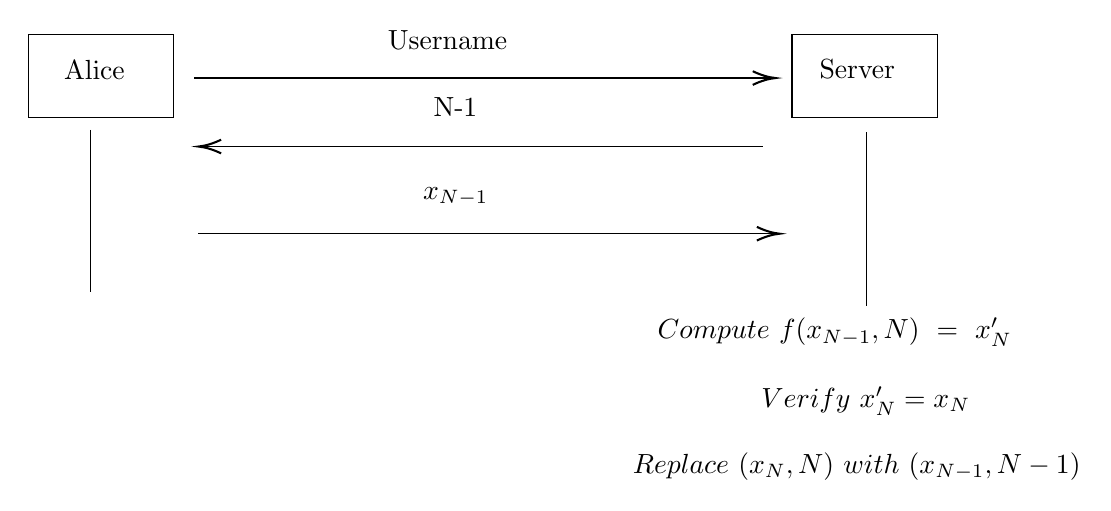
\begin{tikzpicture}[x=0.75pt,y=0.75pt,yscale=-1,xscale=1]
    %uncomment if require: \path (0,300); %set diagram left start at 0, and has height of 300

    %Shape: Rectangle [id:dp9302056250655825] 
    \draw   (108,32) -- (178,32) -- (178,72) -- (108,72) -- cycle ;

    %Shape: Rectangle [id:dp8316101362016359] 
    \draw   (476,32) -- (546,32) -- (546,72) -- (476,72) -- cycle ;

    %Straight Lines [id:da8540576995480886] 
    \draw    (188,53) -- (466,53) ;
    \draw [shift={(468,53)}, rotate = 180] [color={rgb, 255:red, 0; green, 0; blue, 0 }  ][line width=0.75]    (10.93,-3.29) .. controls (6.95,-1.4) and (3.31,-0.3) .. (0,0) .. controls (3.31,0.3) and (6.95,1.4) .. (10.93,3.29)   ;
    %Straight Lines [id:da9236128666658007] 
    \draw    (138,78) -- (138,156) ;
    %Straight Lines [id:da4298900090363067] 
    \draw    (512,79) -- (512,163) ;
    %Straight Lines [id:da6626236203364586] 
    \draw    (462,86) -- (192,86) ;
    \draw [shift={(190,86)}, rotate = 360] [color={rgb, 255:red, 0; green, 0; blue, 0 }  ][line width=0.75]    (10.93,-3.29) .. controls (6.95,-1.4) and (3.31,-0.3) .. (0,0) .. controls (3.31,0.3) and (6.95,1.4) .. (10.93,3.29)   ;
    %Straight Lines [id:da41522984839829913] 
    \draw    (190,128) -- (468,128) ;
    \draw [shift={(470,128)}, rotate = 180] [color={rgb, 255:red, 0; green, 0; blue, 0 }  ][line width=0.75]    (10.93,-3.29) .. controls (6.95,-1.4) and (3.31,-0.3) .. (0,0) .. controls (3.31,0.3) and (6.95,1.4) .. (10.93,3.29)   ;

    % Text Node
    \draw (124,43) node [anchor=north west][inner sep=0.75pt]   [align=left] {Alice};
    % Text Node
    \draw (488,43) node [anchor=north west][inner sep=0.75pt]   [align=left] {Server};
    % Text Node
    \draw (280,29) node [anchor=north west][inner sep=0.75pt]   [align=left] {Username};
    % Text Node
    \draw (302,61) node [anchor=north west][inner sep=0.75pt]   [align=left] {N-1};
    % Text Node
    \draw (297,104.4) node [anchor=north west][inner sep=0.75pt]    {$x_{N-1}$};
    % Text Node
    \draw (410,167.4) node [anchor=north west][inner sep=0.75pt]    {$Compute\ f( x_{N-1} ,N) \ =\ x'_{N}$};
    % Text Node
    \draw (460,200.4) node [anchor=north west][inner sep=0.75pt]    {$Verify\ x'_{N} =x_{N}$};
    % Text Node
    \draw (398,232.4) node [anchor=north west][inner sep=0.75pt]    {$Replace\ ( x_{N} ,N) \ with\ ( x_{N-1} ,N-1)$};

    \end{tikzpicture}

    \caption{Authentication protocol.(Exercise 8)}\label{fig:password_protocol}

\end{figure}

\subsection*{a) Advantages over using ordinary passwords}
%

\begin{itemize}
    \item Easy to detect if an attacker unauthorizedly use your password
    to access the server: Since the server would replace the values
    \((x_N,N)\) with the values \(x_(N-1),N-1\) after each successful
    user authentication, when the server request for the value \emph{N-1}
    which you don't have, that's a moment you realize that someone did
    attack your password (in this case the attacker just passively explore
    what can do with your account without changing your password).

\end{itemize}

\subsection*{b) Possible attacks}
%
\begin{itemize}
    \item Man-in-The-Middle attack is efforlessly conducted since all messages are
    not encrypted.
\end{itemize}

\section*{Exercise 9 --- Functional Encryption}
%
The new NISEC protocol is illustrated in \autoref{fig:nisec_scheme}
\begin{figure}
    \centering

    \tikzset{every picture/.style={line width=0.75pt}} %set default line width to 0.75pt        

    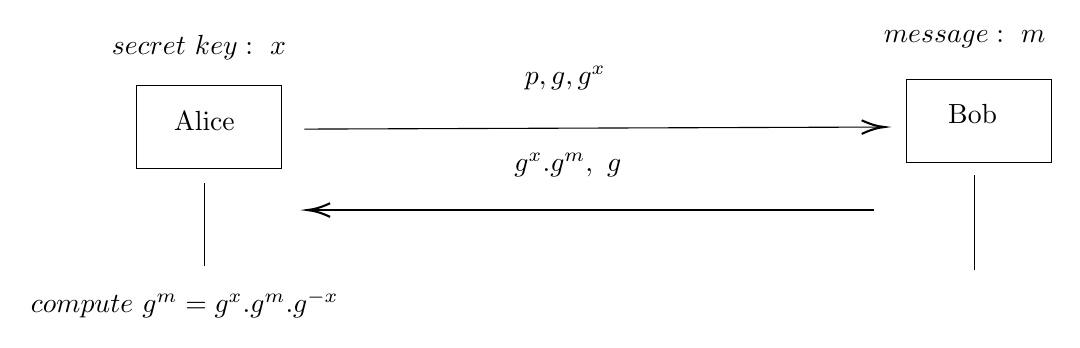
\begin{tikzpicture}[x=0.75pt,y=0.75pt,yscale=-1,xscale=1]
    %uncomment if require: \path (0,181); %set diagram left start at 0, and has height of 181

    %Shape: Rectangle [id:dp22737212763642367] 
    \draw   (95,32) -- (165,32) -- (165,72) -- (95,72) -- cycle ;

    %Shape: Rectangle [id:dp5854265454101574] 
    \draw   (466,29) -- (536,29) -- (536,69) -- (466,69) -- cycle ;

    %Straight Lines [id:da2877686107509583] 
    \draw    (176,53) -- (453.5,52.01) ;
    \draw [shift={(455.5,52)}, rotate = 179.8] [color={rgb, 255:red, 0; green, 0; blue, 0 }  ][line width=0.75]    (10.93,-3.29) .. controls (6.95,-1.4) and (3.31,-0.3) .. (0,0) .. controls (3.31,0.3) and (6.95,1.4) .. (10.93,3.29)   ;
    %Straight Lines [id:da7116831290080069] 
    \draw    (128,79) -- (128,119) ;
    %Straight Lines [id:da19342470100111897] 
    \draw    (499,75) -- (499,121) ;
    %Straight Lines [id:da2580219434326909] 
    \draw    (450.5,92) -- (179.5,92) ;
    \draw [shift={(177.5,92)}, rotate = 360] [color={rgb, 255:red, 0; green, 0; blue, 0 }  ][line width=0.75]    (10.93,-3.29) .. controls (6.95,-1.4) and (3.31,-0.3) .. (0,0) .. controls (3.31,0.3) and (6.95,1.4) .. (10.93,3.29)   ;

    % Text Node
    \draw (112,43) node [anchor=north west][inner sep=0.75pt]   [align=left] {Alice};
    % Text Node
    \draw (485,40) node [anchor=north west][inner sep=0.75pt]   [align=left] {Bob};
    % Text Node
    \draw (281,21.4) node [anchor=north west][inner sep=0.75pt]    {$p,g,g^{x}$};
    % Text Node
    \draw (276,63.4) node [anchor=north west][inner sep=0.75pt]    {$g^{x} .g^{m} ,\ g$};
    % Text Node
    \draw (82,6.4) node [anchor=north west][inner sep=0.75pt]    {$secret\ key:\ x$};
    % Text Node
    \draw (454,4.4) node [anchor=north west][inner sep=0.75pt]    {$message:\ m$};
    % Text Node
    \draw (43,129.4) node [anchor=north west][inner sep=0.75pt]    {$compute\ g^{m} =g^{x} .g^{m} .g^{-x}$};

    \end{tikzpicture}

    \caption{New NISEC encryption scheme.(Exercise 9)}\label{fig:nisec_scheme}
\end{figure}

\subsection*{a) Drawbacks of the new encryption scheme}
%
\begin{itemize}
    \item \textbf{Lack of data integrity}: HMAC should be implemented on top of the
    public parammeters to make sure they were not intercepted.
    \item \textbf{Lack of mutual authentication}: there is no authentication protocol between
    the sender and the receiver, so it very easy for an attacker to intervene the 
    connection.
    \item \textbf{Resource expensive algorithms}: using public key cryptography to
    encrypt/decrypt the long message takes lots of time and computational
    resources. Instead, symmetric cryptography should be used to avoid 
    operating on enormous prime numbers. The asymmetric cryptography, public key
    cryptography, can be used to encrypt the symmetric key. Then the encrypted
    key is utilized to encrypt/decrypt a long message (a large file).
\end{itemize}

Some possible attacks are illustrated in \autoref{fig:imp_receiver} and \autoref{fig:imp_sender}:

\begin{figure}
    \centering

    \tikzset{every picture/.style={line width=0.75pt}} %set default line width to 0.75pt        

    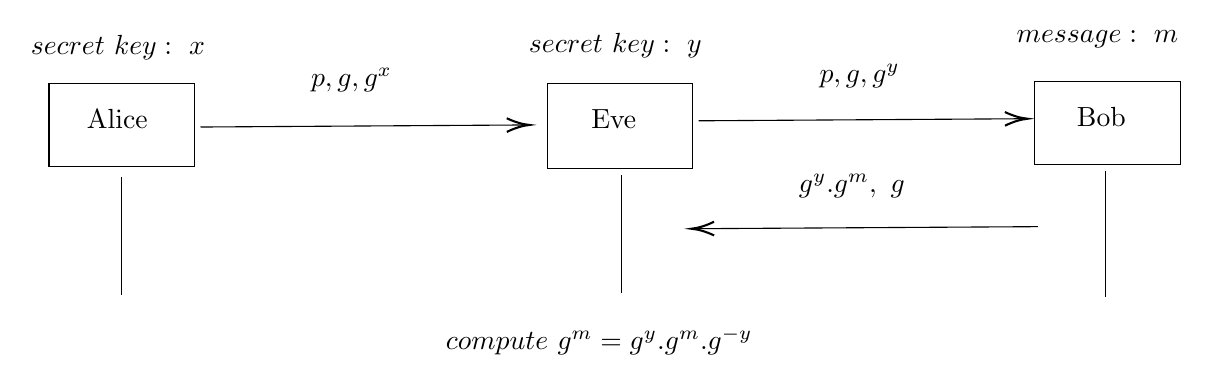
\begin{tikzpicture}[x=0.75pt,y=0.75pt,yscale=-1,xscale=1]
    %uncomment if require: \path (0,234); %set diagram left start at 0, and has height of 234

    %Shape: Rectangle [id:dp6501223431872357] 
    \draw   (54,70) -- (124,70) -- (124,110) -- (54,110) -- cycle ;

    %Shape: Rectangle [id:dp8447479220950903] 
    \draw   (529,69) -- (599,69) -- (599,109) -- (529,109) -- cycle ;

    %Straight Lines [id:da3587916713070962] 
    \draw    (127,91) -- (283.5,90.01) ;
    \draw [shift={(285.5,90)}, rotate = 179.64] [color={rgb, 255:red, 0; green, 0; blue, 0 }  ][line width=0.75]    (10.93,-3.29) .. controls (6.95,-1.4) and (3.31,-0.3) .. (0,0) .. controls (3.31,0.3) and (6.95,1.4) .. (10.93,3.29)   ;
    %Straight Lines [id:da12630867495123377] 
    \draw    (89,115) -- (89,172) ;
    %Straight Lines [id:da07235943303271719] 
    \draw    (563,112) -- (563,173) ;
    %Straight Lines [id:da044820189761365814] 
    \draw    (530.5,139) -- (365.5,139.99) ;
    \draw [shift={(363.5,140)}, rotate = 359.66] [color={rgb, 255:red, 0; green, 0; blue, 0 }  ][line width=0.75]    (10.93,-3.29) .. controls (6.95,-1.4) and (3.31,-0.3) .. (0,0) .. controls (3.31,0.3) and (6.95,1.4) .. (10.93,3.29)   ;
    %Shape: Rectangle [id:dp8175805944937183] 
    \draw   (294,70) -- (364,70) -- (364,111) -- (294,111) -- cycle ;

    %Straight Lines [id:da4400636896192306] 
    \draw    (367,88) -- (523.5,87.01) ;
    \draw [shift={(525.5,87)}, rotate = 179.64] [color={rgb, 255:red, 0; green, 0; blue, 0 }  ][line width=0.75]    (10.93,-3.29) .. controls (6.95,-1.4) and (3.31,-0.3) .. (0,0) .. controls (3.31,0.3) and (6.95,1.4) .. (10.93,3.29)   ;
    %Straight Lines [id:da8522907791652553] 
    \draw    (330,114) -- (330,171) ;

    % Text Node
    \draw (179,61.4) node [anchor=north west][inner sep=0.75pt]    {$p,g,g^{x}$};
    % Text Node
    \draw (414,112.4) node [anchor=north west][inner sep=0.75pt]    {$g^{y} .g^{m} ,\ g$};
    % Text Node
    \draw (44,45.4) node [anchor=north west][inner sep=0.75pt]    {$secret\ key:\ x$};
    % Text Node
    \draw (519,43.4) node [anchor=north west][inner sep=0.75pt]    {$message:\ m$};
    % Text Node
    \draw (244,186.4) node [anchor=north west][inner sep=0.75pt]    {$compute\ g^{m} =g^{y} .g^{m} .g^{-y}$};
    % Text Node
    \draw (548,80) node [anchor=north west][inner sep=0.75pt]   [align=left] {Bob};
    % Text Node
    \draw (71,81) node [anchor=north west][inner sep=0.75pt]   [align=left] {Alice};
    % Text Node
    \draw (314,81.49) node [anchor=north west][inner sep=0.75pt]   [align=left] {Eve};
    % Text Node
    \draw (424,59.4) node [anchor=north west][inner sep=0.75pt]    {$p,g,g^{y}$};
    % Text Node
    \draw (284,44.4) node [anchor=north west][inner sep=0.75pt]    {$secret\ key:\ y$};

    \end{tikzpicture}

    \caption{The attacker impersonates the receiver.(Exercise 9)}\label{fig:imp_receiver}
\end{figure}

\begin{figure}
    \centering


    \tikzset{every picture/.style={line width=0.75pt}} %set default line width to 0.75pt        

    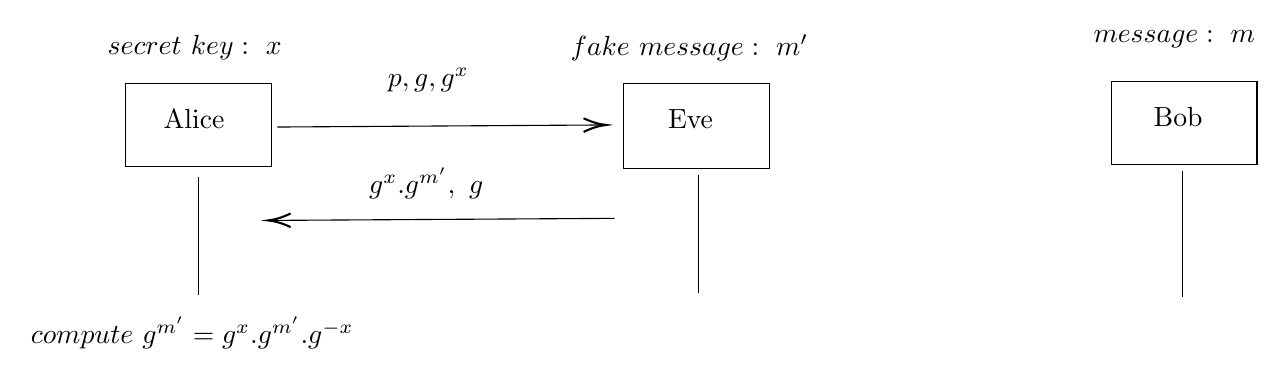
\begin{tikzpicture}[x=0.75pt,y=0.75pt,yscale=-1,xscale=1]
    %uncomment if require: \path (0,300); %set diagram left start at 0, and has height of 300

    %Shape: Rectangle [id:dp1403171227510649] 
    \draw   (74,90) -- (144,90) -- (144,130) -- (74,130) -- cycle ;

    %Shape: Rectangle [id:dp6601513404208796] 
    \draw   (549,89) -- (619,89) -- (619,129) -- (549,129) -- cycle ;

    %Straight Lines [id:da9197769654145035] 
    \draw    (147,111) -- (303.5,110.01) ;
    \draw [shift={(305.5,110)}, rotate = 179.64] [color={rgb, 255:red, 0; green, 0; blue, 0 }  ][line width=0.75]    (10.93,-3.29) .. controls (6.95,-1.4) and (3.31,-0.3) .. (0,0) .. controls (3.31,0.3) and (6.95,1.4) .. (10.93,3.29)   ;
    %Straight Lines [id:da9223813286436544] 
    \draw    (109,135) -- (109,192) ;
    %Straight Lines [id:da34247791753331325] 
    \draw    (583,132) -- (583,193) ;
    %Straight Lines [id:da7861276918756701] 
    \draw    (309.5,155) -- (144.5,155.99) ;
    \draw [shift={(142.5,156)}, rotate = 359.66] [color={rgb, 255:red, 0; green, 0; blue, 0 }  ][line width=0.75]    (10.93,-3.29) .. controls (6.95,-1.4) and (3.31,-0.3) .. (0,0) .. controls (3.31,0.3) and (6.95,1.4) .. (10.93,3.29)   ;
    %Shape: Rectangle [id:dp488004334450037] 
    \draw   (314,90) -- (384,90) -- (384,131) -- (314,131) -- cycle ;

    %Straight Lines [id:da988601175202231] 
    \draw    (350,134) -- (350,191) ;

    % Text Node
    \draw (199,81.4) node [anchor=north west][inner sep=0.75pt]    {$p,g,g^{x}$};
    % Text Node
    \draw (190,129.4) node [anchor=north west][inner sep=0.75pt]    {$g^{x} .g^{m'} ,\ g$};
    % Text Node
    \draw (64,65.4) node [anchor=north west][inner sep=0.75pt]    {$secret\ key:\ x$};
    % Text Node
    \draw (539,63.4) node [anchor=north west][inner sep=0.75pt]    {$message:\ m$};
    % Text Node
    \draw (27,201.4) node [anchor=north west][inner sep=0.75pt]    {$compute\ g^{m'} =g^{x} .g^{m'} .g^{-x}$};
    % Text Node
    \draw (287,65.4) node [anchor=north west][inner sep=0.75pt]    {$fake\ message:\ m'$};
    % Text Node
    \draw (334,101.49) node [anchor=north west][inner sep=0.75pt]   [align=left] {Eve};
    % Text Node
    \draw (568,100) node [anchor=north west][inner sep=0.75pt]   [align=left] {Bob};
    % Text Node
    \draw (91,101) node [anchor=north west][inner sep=0.75pt]   [align=left] {Alice};


    \end{tikzpicture}

    \caption{The attacker impersonates the sender.(Exercise 9)}\label{fig:imp_sender}
\end{figure}

\subsection*{b) Linear cihpertext homomorphic and linear key homomorphic}
%
The notation \(Enc(pk_i, x_i)=g^{sk_i}\cdot g^{x_i}\) is used to denote the encryption of the
message \(x_i\) using the public key \(pk_i\).

\textbf{Prove that the scheme is linear ciphertext homomorphic}\\

The linear ciphertext homomorphic property is then:
\begin{align*}
    Enc(pk_1, x_1) \cdot...\cdot Enc(pk_n, x_n) &= (g^{sk_1}\cdot g^{x_1})
    \cdot...\cdot(g^{sk_n}\cdot g^{x_n})\\
    &= (g^{sk_1}\cdot...\cdot g^{sk_n})\cdot(g^{x_1}\cdot...\cdot g^{x_n})\\
    &= g^{sk_1+\cdots +sk_n}\cdot g^{x_1+\cdots +x_n}\\
    &= Enc(pk_1\cdot...\cdot pk_n, x_1+\cdots +x_n)
\end{align*}

\textbf{Prove that the scheme is linear key homomorphic}\\
Given \emph{n} public/private key pairs:\\
\begin{align*}
    (pk_1,sk_1),\cdots,(pk_n,sk_n),
\end{align*}

for each key pair the following expression holds:
\begin{align*}
    &pk_i,sk_i\\
    \Leftrightarrow &g^{sk_i},sk_i.
\end{align*}

Using a newly constructed key pair:

\begin{align*}
    &pk_1\cdot...\cdot pk_n, sk_1+...+ sk_n\\
    \Leftrightarrow &g^{sk_1}\cdot...\cdot g^{sk_n}, sk_1+...+ sk_n\\
    \Leftrightarrow &g^{sk_1+...+sk_n}, sk_1+...+sk_n.
\end{align*}

Thus, the new key pair is valid, so the linear key homomorphic property holds.

\subsection*{c) Explain how the CSP can compute \(x_1+\cdots+x_n\)}
%
The CSP already know the sum of secret keys:
\begin{align*}
    sk_1+\cdots+sk_n,
\end{align*}
and given each ciphertext \(c_i\), it can compute the product of all uploaded ciphertext:
\begin{align*}
    c_1\cdot...\cdot c_n &= g^{(sk_1+x_1)+\cdots +(sk_n+x_n)}\\
    &= g^{(sk_1+\cdots +sk_n)+(x_1+\cdots +x_n)}\\
    &= g^{sk_1+\cdots +sk_n}\cdot g^{x_1+\cdots +x_n},    
\end{align*}

through these data, it can compute:
\begin{align*}
    g^{x_1+\cdots +x_n} &= \frac{c_1\cdot...\cdot c_n}{g^{sk_1+\cdots +sk_n}}\\
    &= K.
\end{align*}

The sum of all plaintexts can be retrieved by:
\begin{align*}
    x_1+\cdots+x_n &= \log_{g}K. (discrete\ logarithm\ problem)
\end{align*}

\section*{Exercise 10 --- Key Distribution}
%

\section*{Bonus Exercise}
%

\printbibliography

\end{document}